\subsection{Реализация генератора изображений captcha для создания большого объема данных}
Как известно, для обучения сверточных нейронных сетей необходимы значительные объемы данных. В нашем случае, мы будем проводить обучение решающей сети на 200,000 изображений captcha, причем каждому изображению должен быть присвоен ожидаемый ответ. Создание такого датасета из реальных данных вручную потребовало бы траты большого количества ресурсов и времени, учитывая, что среднее время, затрачиваемое человеком на решение одной картинки captcha – 10 секунд. Еще один недостаток ручного метода – наличие определенного процента ошибок.

Вместо того, чтобы создавать этот датасет вручную, мы будем генерировать изображения captcha искусственно, с заранее известным ответом, что исключает необходимость вмешательства человека. Вместе с тем, искусственно созданные изображения должны быть максимально похожи на картинки целевого сайта.

Стоит отметить, что на следующем шаге, во время обучения Pix2Pix сети, которая должна очищать изображение от защитных средств (шум, линии, искажения), нам понадобится датасет, состоящий из входных изображений – captcha с защитными средствами и ожидаемых изображений – стандартизированных версий картинок без защитных средств. Создание такого набора данных, состоящего из пар входных и выходных изображений, тоже было бы невозможно в случае ручной обработки данных.

Генератор искусственных изображений состоит из двух частей. Сначала создается изображение, приблизительно похожее на картинки из реального датасета, полученного на предыдущем шаге. На этом же шаге генератор создает изображение без защитных средств, которое мы в дальнейшем будем использовать для обучения Pix2Pix сети. После этого изображение направляется в simGAN сеть, которая производит модифицаию изображения на пиксельном уровне, делая искусственно созданные изображения практически неотличимыми от настоящих.

Рассмотрим реальные изображения из датасета, созданного на предыдущем шаге. В силу того, что в нашем случае цвет не несет в себе полезных данных, а лишь усложняет модели, все изображения были конвертированы в монохром.

Выделим защитные средства, использующиеся в целевых изображениях:
\begin{itemize}
	\item фон состоит из размытых полос, расположенных в случайном направлении;
	\item позади текста находится около 5 темных линий случайной формы;
	\item символы текста находятся на разных уровнях и повернуты на случайный угол;
	\item ко всему изображению применена дисторсия произвольного направления.
	
\end{itemize}

Приступим к реализации генератора на языке php с использованием библиотеки Imagick.
Чтобы сделать фон с полосами, достаточно расположить линии через случайный интервал в произвольном направлении и применить размытие. В листинге \ref{lst:captcha-gen-lines-bg} приводится реализация этой идеи. Последующие применения дисторсии к изображению сделают полосы более хаотичными и похожими на оригинал.

\begin{lstlisting}[language=PHP,basicstyle=\fontsize{11}{11}\selectfont,tabsize=4,breaklines=true,caption={Отрисовка размытых линий для фона.},captionpos=b,label={lst:captcha-gen-lines-bg}]
$lineStart = rand(0, $width);
$lineCoords = [$lineStart, 0, $lineStart + rand(-50, 50), $height];
$bgLines = new ImagickDraw();
$bgLines->setStrokeWidth(1);
$bgLines->setStrokeColor(new ImagickPixel('#e1e1e1'));
$bgLines->line($lineCoords[0], $lineCoords[1], $lineCoords[2], $lineCoords[3]);
$step = rand(8, 18);
for ($offset = $step; $offset < 150; $offset += $step) {
	$bgLines->line($lineCoords[0] - $offset, $lineCoords[1], $lineCoords[2] - $offset, $lineCoords[3]);
	$bgLines->line($lineCoords[0] + $offset, $lineCoords[1], $lineCoords[2] + $offset, $lineCoords[3]);
}
$image->drawImage($bgLines);
$image->blurImage(3, 3);
\end{lstlisting}

На рисунке \ref{fig:cgen-1} изображен получившийся фон с размытыми линиями.
\begin{figure}[h]
	\centering
	
\includegraphics[width=0.3\textwidth]{cgen-1}
	\caption{Результат работы генератора на первом этапе.}
	\label{fig:cgen-1}
\end{figure}

Темные линии случайной формы могут быть получены размещением произвольного числа линий (до 5 в нашем случае) и применением дисторсии в случайных точках по методу shepard -- см. листинг \ref{lst:captcha-gen-lines-dark}.
\begin{lstlisting}[language=PHP,basicstyle=\fontsize{11}{11}\selectfont,tabsize=4,breaklines=true,caption={Генерирование темных линий и применение дисторсии.},captionpos=b,label={lst:captcha-gen-lines-dark}]
$linesCount = rand(2, 5);

$randomPoint = [rand(30, $width - 30), rand(15, $height - 15)];

$minD = 10;
$maxD = 30;
$points = [
	rand(0, $width), rand(0, $height),
	// ...
];
$image->setImageVirtualPixelMethod(Imagick::VIRTUALPIXELMETHOD_EDGE);

for ($i = 0; $i < $linesCount; $i++) {
	$image->drawImage(getRandomLine());
}

$image->distortImage(Imagick::DISTORTION_SHEPARDS, $points, true);
\end{lstlisting}

Результат генерирования темных линий приводится на рисунке \ref{fig:cgen-2}.
\begin{figure}[h]
	\centering
	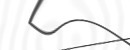
\includegraphics[width=0.3\textwidth]{cgen-2}
	\caption{Создание темных линий.}
	\label{fig:cgen-2}
\end{figure}

Для отрисовки текста воспользуемся шрифтом Source Serif. Сначала генерируется случайное слово из допустимых символов заданной длины. После чего на картинку посимвольно наносится текст. Угол поворота, положение и расстояние между символами выбираются случайным образом на каждой итерации. Эти действия выполнены в листинге \ref{lst:captcha-gen-word}.
\begin{lstlisting}[language=PHP,basicstyle=\fontsize{11}{11}\selectfont,tabsize=4,breaklines=true,caption={Отрисовка случайного слова.},captionpos=b,label={lst:captcha-gen-word}]
$word = random_str(6, '24578acdehjkmnpqsuvwxyz');

$drawSettings = new ImagickDraw();
$drawSettings->setFont($fontName);
$drawSettings->setFontSize(36);
$drawSettings->setFillColor(new ImagickPixel('black'));
$drawSettings->setStrokeColor(new ImagickPixel('#acacac'));
$drawSettings->setStrokeWidth(0.3);

$x = rand(8, 12);
for ($i = 0; $i < strlen($word); $i++) {
	$drawSettings->setFillColor(new ImagickPixel('graya(' . rand(15, 35) . '%, 1)'));
	$angle = rand(0, 5);
	$image->annotateImage($drawSettings, $x, rand(26, 34), $angle, $word[$i]);
	$box = imagettfbbox(28, $angle, $fontName, $word[$i]);
	$charWidth = abs($box[0]) + abs($box[2]);
	$x += rand($charWidth - 7, $charWidth);
}
\end{lstlisting}

На рисунке \ref{fig:cgen-3} -- изображение captcha, созданное на текущем этапе.
\begin{figure}[h]
	\centering
	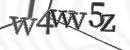
\includegraphics[width=0.3\textwidth]{cgen-3}
	\caption{Результат отображения случайного слова.}
	\label{fig:cgen-3}
\end{figure}

Остается добавить дисторсию к буквам. В ходе разработки было выяснено, что задание опорных точек дисторсии полностью случайным образом иногда приводит к появлению артефактов и неразгадываемой captcha, поэтому генератор использует набор предопределенных опорных точек и выбирает один случайный шаблон. Реализация последнего этапа создания изображения приводится в листинге \ref{lst:captcha-gen-distortion}.
\begin{lstlisting}[language=PHP,basicstyle=\fontsize{11}{11}\selectfont,tabsize=4,breaklines=true,caption={Применение дисторсии.},captionpos=b,label={lst:captcha-gen-distortion}]
$points = [
	[
		40, 25,
		40, 30,
		// ...
	],
	// ...
];

$image->distortImage(Imagick::DISTORTION_SHEPARDS, $points[array_rand($points)], true);

$image->writeImage($fileName);
\end{lstlisting}

Итоговый результат работы генератора приводится на изображении \ref{fig:cgen-4}.
\begin{figure}[h]
	\centering
	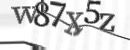
\includegraphics[width=0.3\textwidth]{cgen-4}
	\caption{Результат применения дисторсии.}
	\label{fig:cgen-4}
\end{figure}

Сравним картинки, полученные при помощи генератора с исходными данными (Рис. \ref{fig:cgen-comparison}). Сверху -- картинки из исходного датасета, снизу -- изображения, полученные при помощи генератора.
\begin{figure}[h]
	\centering
	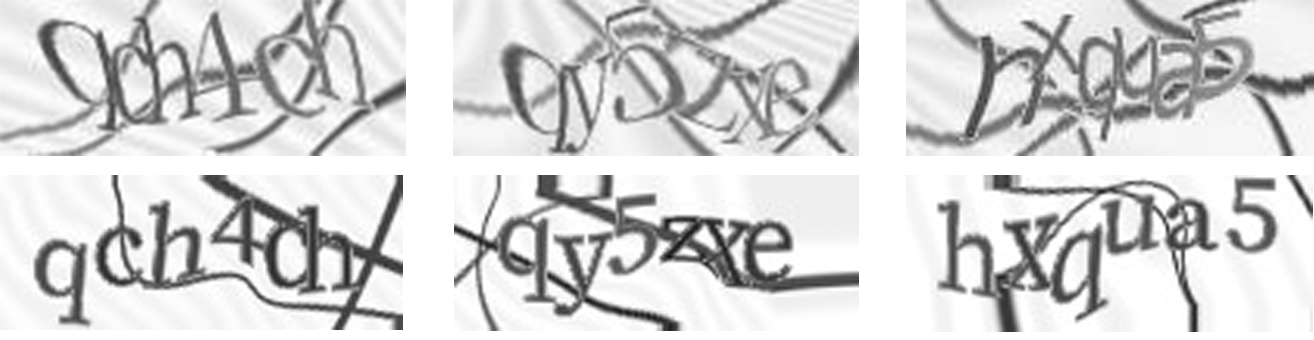
\includegraphics[width=0.8\textwidth]{cgen-comparison}
	\caption{Сравнение исходных изображений с искусственно созданными.}
	\label{fig:cgen-comparison}
\end{figure}